\documentclass{article}
\usepackage{amsfonts}
\usepackage{amsmath}
\usepackage{mathtools}
\usepackage{systeme}
\usepackage{polynom}
\usepackage{pgfplots}
\usepackage[shortlabels]{enumitem}
\usepackage[a4paper,margin=1in,footskip=0.25in]{geometry}
\everymath{\displaystyle}
\DeclarePairedDelimiter\ceil{\lceil}{\rceil}
\newcommand{\p}[1]{\frac{\partial}{\partial #1}}
\begin{document}
\begin{center}
\Large\textbf{Kodutöö nr. 6}\\
1. variant\\
\small{Joosep Näks}
\end{center}
\textbf{1. }Arendada funktsioon$$f(x)=\frac{\pi}4-\frac x2,\ x\in[0,\pi],$$siinusreaks. Uurida rea punktiviisi koonduvust (s.t. kas koondub ja mis väärtuseks) lõigus $[0,\pi]$.\\
Olgu $s_n(x)$ selle siinusrea n-nes osasumma ning olgu $$\sigma_n(x)=\frac{s_0(x)+...+s_n(x)}{n+1}$$ Joonistada lõigus $[-5,5]$ graafik, millel oleks toodud funktsioonid $f,\ s_{10},\ s_{100}$ ning samas lõigus teine graafik, millel oleks toodud funktsioonid $f,\ \sigma_{10},\ \sigma_{100}$.\\\\
\textbf{Lahendus:}\\
Jätkan funktsiooni $f$ lõigule $[-\pi,\pi]$ paarituks funktsiooniks $\tilde{f}$:
\begin{gather*}
\tilde f(x):=\left\{\begin{aligned}
&f(x)=\frac{\pi}4-\frac x2,&&\text{kui }x\in[0,\pi];\\
&f(x)=-\frac{\pi}4-\frac x2,&&\text{kui }x\in[-\pi,0)
\end{aligned}
\right.
\end{gather*}
Leian $\tilde f$ Fourier' kordajad:
\begin{gather*}
\begin{aligned}
b_n:=&\frac2{\pi}\int_0^{\pi}f(x)\sin kx\ dx\\
=&\frac2{\pi}\int_0^{\pi}\left(\frac{\pi}4-\frac x2 \right)\sin kx\ dx\\
=&\frac2{\pi}\left(-\frac{2\sin(kx)+k(\pi-2x)\cdot\cos(kx)}{4k^2}\right)\Bigg|_0^{\pi}\\
=&\frac2{\pi}\left(\frac{k\pi-2\sin(k\pi)+k\pi\cos(k\pi)}{4k^2}\right)\\
=&\frac{1+(-1)^{k}}{2k}\\
\end{aligned}
\end{gather*}
Ehk $\tilde f \sim \sum_{k=1}^\infty\frac{1+(-1)^k}{2k}\sin kx$ ning kuna lõigus $[0,\pi]$ on $f$ ja $\tilde f$ samad, on saadud Fourier' rida ka funktsiooni $f$ Fourier' rida selles lõigus. Funktsioonil $f$ on punktides $c\in[0,\pi]$ lõplik tuletis seega loengukonspekti järelduse 2.3 kohaselt koondub rida nendes punktides väärtusteks $f(x)$.\\
Osasumma graafikud:
\begin{center}
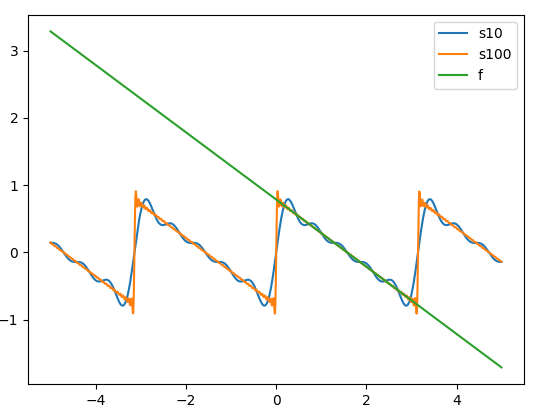
\includegraphics[scale=0.4]{graaf1_mma_6.png}
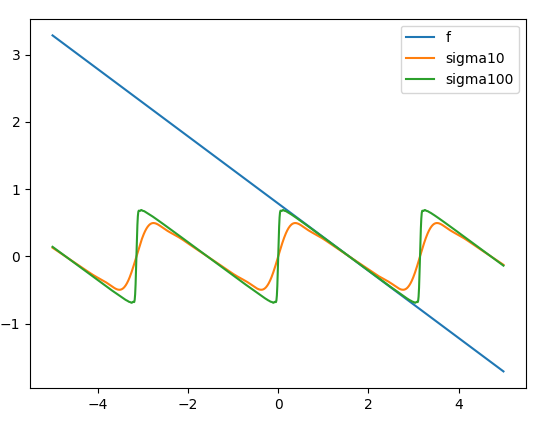
\includegraphics[scale=0.4]{graaf2_mma_6.png}
\end{center}\ 
\pagebreak\\
\textbf{2. } Vaatleme eelmise ülesande funktsiooni $f$ arendise osasummat kujul $$s_m=\sum_{k=0}^mc_k\varphi_k,$$kus $(\varphi_k)$ on trigonomeetriline ortonormeeritud süsteem, s.t. $$\varphi_0(x)=\frac1{\sqrt{2\pi}},\quad\varphi_1(x)=\frac{\cos x}{\sqrt{\pi}},\ \quad\varphi_2(x)=\frac{\sin x}{\sqrt{\pi}},\ \quad\varphi_3(x)=\frac{\cos 2x}{\sqrt{\pi}},\ \quad\varphi_4(x)=\frac{\sin 2x}{\sqrt{\pi}},\ ....$$(siinusrea kordajad ongi konstantse teguriga korrutamise täpsuseni arvud $(c_k)$).\\
Kasutades võrdust $$||f-s_n||^2=||f||^2-\sum_{k=0}^nc^2_k,$$leida vähim selline $n$, et osasumma $s_n$ ja funktsiooni $f$ (täpsemalt, tema paaritu jätku lõigule $[-\pi,\pi]$) ruutkeskmine viga $||f-s_n||$ oleks väiksem kui 0,1.\\\\
\textbf{Lahendus:}\\
Eelmises ülesandes leitud Fourier' kordajate põhjal saan et $c_0=0$ ja $c_{2k-1}=0,\ k\in\mathbb{N}$ ning $c_{2k}=\frac{\sqrt{\pi}(1+(-1)^{\frac k2})}{k},\ k\in\mathbb{N}$. Võrratus $||f-s_n||<0,1$ on samaväärne võrratusega $\sqrt{||f||^2-\sum_{k=0}^nc^2_k}<0,1$ ehk $||f||^2-\sum_{k=0}^nc^2_k<0,01$. $||f||$ saab lahti kirjutada kui: $$||f||=\sqrt{2\int_0^{\pi}\left|\frac{\pi}4-\frac x2\right|^2 dx}=\sqrt{\frac{\pi^3}{24}}$$ Seega on vaja leida vähim $n$ nii, et $$\frac{\pi^3}{24}-\sum_{k=0}^nc_k^2<0.01$$ Programmiga läbi proovides sain, et $n=158$, kuna $\frac{\pi^3}{24}-\sum_{k=0}^{157}c_k^2\approx0.0100$ ning $\frac{\pi^3}{24}-\sum_{k=0}^{158}c_k^2\approx0.0099$.
\end{document}